\documentclass{acmsiggraph}               % final
%\documentclass[review]{acmsiggraph}      % review
%\documentclass[widereview]{acmsiggraph}  % wide-spaced review
%\documentclass[preprint]{acmsiggraph}    % preprint

%% Uncomment one of the four lines above depending on where your paper is
%% in the conference process. ``review'' and ``widereview'' are for review
%% submission, ``preprint'' is for pre-publication, and ``final'' is for
%% the version to be printed.

%% These two line bring in essential packages: ``mathptmx'' for Type 1 
%% typefaces, and ``graphicx'' for inclusion of EPS figures.

\usepackage{mathptmx}
\usepackage{graphicx}

%% use this for zero \parindent and non-zero \parskip, intelligently.

\usepackage{parskip}

%% If you are submitting a paper to the annual conference, please replace 
%% the value ``0'' below with your OnlineID. If you are not submitting this
%% paper to the annual conference, you may safely leave it at ``0'' -- it 
%% will not be included in the output.

\onlineid{0}

%% need to document this!

\acmformat{print}

%% Paper title.

\title{Digital Circuit Sketch Recognition}

%% Author and Affiliation (single author).

%\author{Jason Fennell\\Harvey Mudd College\\jfennell@hmc.edu
%\and Max Pflueger\\Harvey Mudd College\\mpflueger@hmc.edu
%\and Devin Smith\\Harvey Mudd College\\jfennell@hmc.edu
%\and Aaron Wolin\\Harvey Mudd College\\awolin@hmc.edu
%\and Christine Alvarado\\Harvey Mudd College\\alvarado@hmc.edu}


\author{Jason Fennell, Max Pflueger, Devin Smith, Aaron Wolin, Christine Alvarado\\Harvey Mudd College\\\{jfennell,mpflueger,dsmith,awolin,alvarado\}@hmc.edu}

%% Keywords that describe your work.

\keywords{}

%%%%%% START OF THE PAPER %%%%%%

\begin{document}

%% The ``\maketitle'' command must be the first command after the
%% ``\begin{document}'' command. It prepares and prints the title block.

\maketitle

\section*{Toolchain Summary}

The toolchain begins with a sketch being input into Microsoft Journal
Reader and saved as a .jnt file.  This .jnt is passed through a
converter to change it into the MIT XML format that our group uses.
The sketch is now ready to go through the actual meat of the
toolchain.  The sketch is first fragmented into lines and arcs to give
us more strokes to train on, and simpler strokes to recognize.  For
more information on the fragmentation, see the report by Aaron Wolin
\cite{wolin:fragmenter}.  The fragmented sketch is next passed into a
Conditional Random Field for recognition of the individual strokes.
For more information on the stroke-level recognition, see the report
by Jason Fennell and Max Pflueger \cite{fennellPflueger:CRF}.  Once
stroke-level recognition has finished, another program called a
segmenter uses the recognized strokes to segment our drawing into
logical components by grouping sets of strokes that make up gates or
wires together.  This segmenter goes back and forth with a shape
recognizer that attempts to recognize the components.  For more
information on segmentation and shape recognition, see the report by
Devin Smith \cite{smith:segmentation}.  Once this final recognition
step is complete, the circuit undergoes analysis and is passed to a
design program, fully understood by the computer.

\section*{Example}

This section shows an example of our toolchain in its current state.

In Figure \ref{journal} we see the digital circuit just after it has been finished.  
It is ready to go through the toolchain.

\begin{figure}[p]
\centering
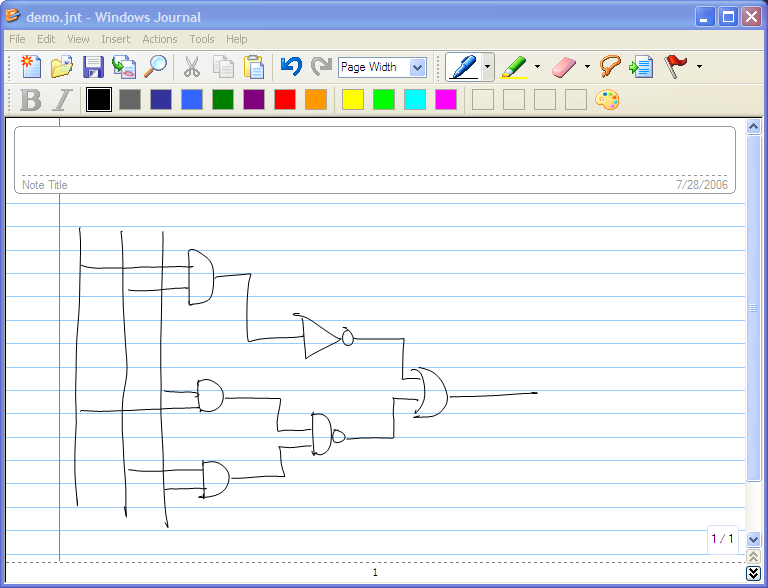
\includegraphics[width=1.8in]{sketchInJournal.png}
\caption{Sketch being drawn}
\label{journal}
\end{figure}

In Figure \ref{fragmented} we see the fragmented circuit.
Note the wire between the AND and NAND with the selected stroke.  
This wire was drawn in one motion, but has been broken up into line segments by our fragmenter.


\begin{figure}[p]
\centering
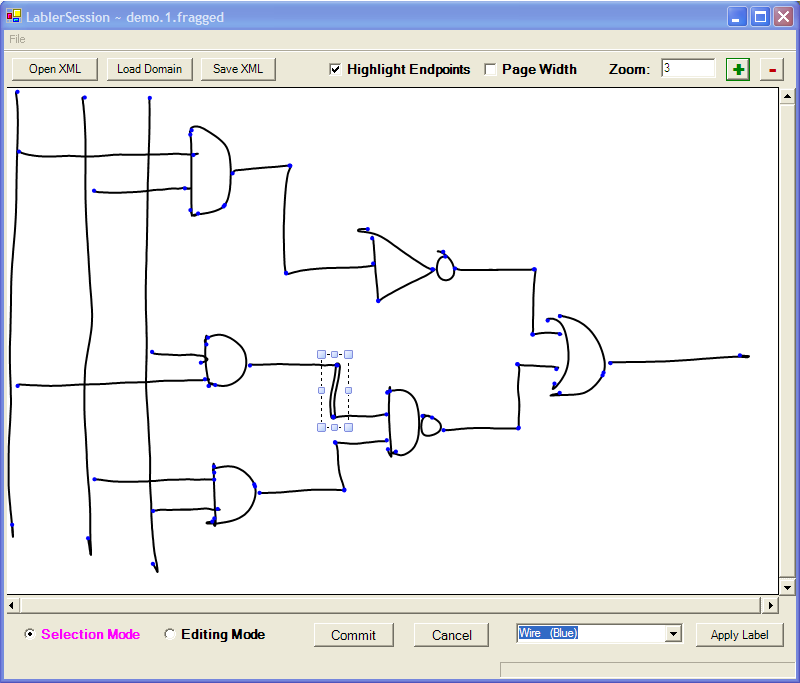
\includegraphics[width=1.8in]{fragmentedSketch.png}
\caption{Sketch after conversion to XML and fragmentation}
\label{fragmented}
\end{figure}

In Figure \ref{CRFed} we see the circuit after stroke-level recognition.  
Red strokes have been classified as part of a gate and blue ones as part of a wire.  
Note that only one stroke, the backplane at the far left of the diagram, was misclassified.

\begin{figure}[p]
\centering
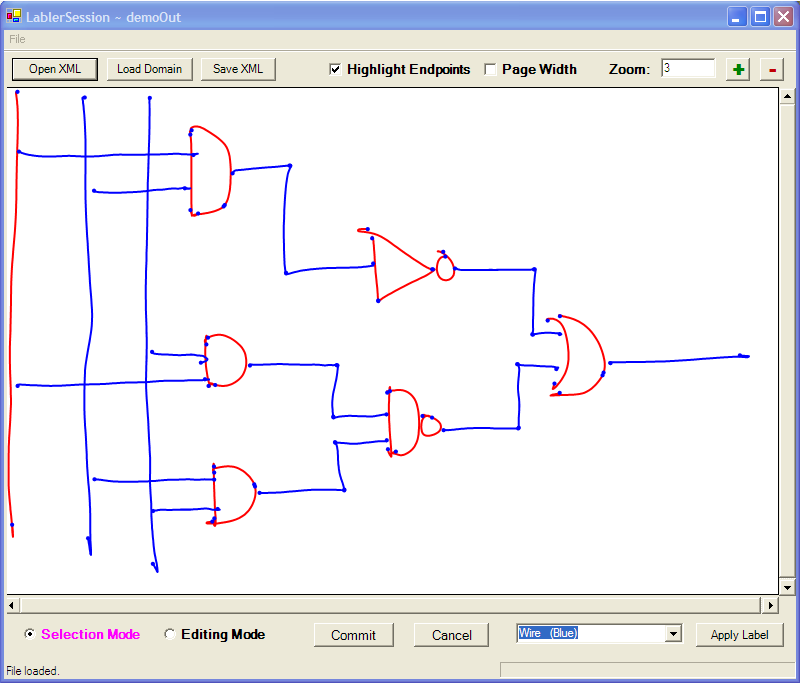
\includegraphics[width=1.8in]{classifiedSketch.png}
\caption{Sketch after stroke-level recognition}
\label{CRFed}
\end{figure}

In Figure \ref{segmented} we see the segmented circuit.  
Each different color indicates a group of strokes that have been placed together in a component.  
Note that the only error in the segmentation is with the wires connected to the misclassified backplane from Figure \ref{CRFed}.  
The backplane and the two wires connected two it are all segmented as different components when they should not be.

\begin{figure}[p]
\centering
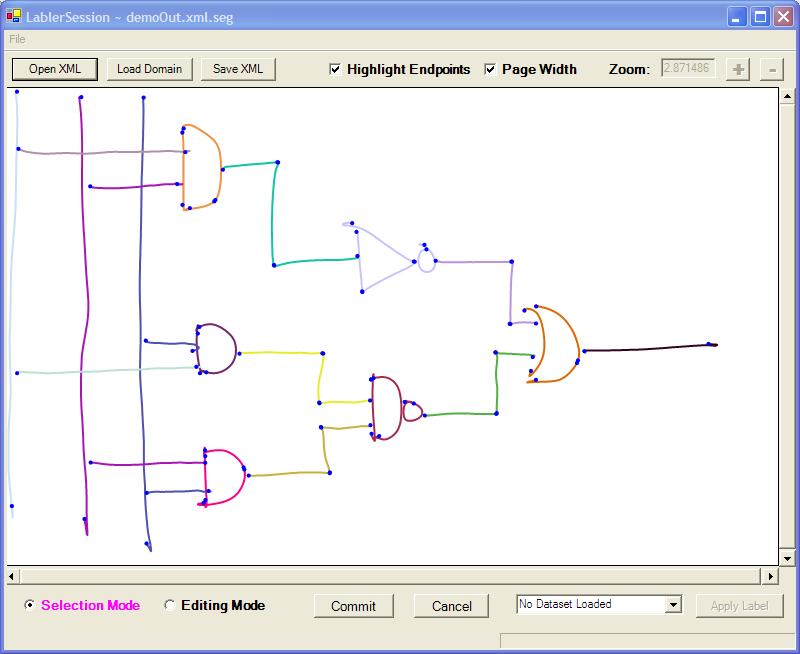
\includegraphics[width=1.8in]{segmentedSketch.png}
\caption{Sketch after segmentation}
\label{segmented}
\end{figure}


\bibliographystyle{acmsiggraph}
\nocite{*}
\bibliography{SketchRecognition}
\end{document}

